% document class and packages
\documentclass[12pt, titlepage]{article}
\usepackage{pgfgantt}
\usepackage{geometry}
\usepackage{graphicx}
\usepackage{rotating}
\usepackage[nottoc,numbib]{tocbibind}

% settings
\geometry{a4paper, total={170mm,257mm}, left=25mm,
right=25mm, top=20mm, bottom=20mm}
\setlength{\parindent}{0em}
\setlength{\parskip}{1em}


% document begins here
\begin{document}
\begin{titlepage} % Suppresses displaying the page number on the title page and the subsequent page counts as page 1
	\newcommand{\HRule}{\rule{\linewidth}{0.5mm}} % Defines a new command for horizontal lines, change thickness here

	\center % Centre everything on the page

	%------------------------------------------------
	%	Headings
	%------------------------------------------------

	\textsc{\LARGE Queen Mary University of London}\\[1.5cm] % Main heading such as the name of your university/college
	\textsc{\Large Final Year Project Specification}\\[0.5cm] % Major heading such as course name
	\textsc{\large Session 2017/2018}\\[0.5cm] % Minor heading such as course title

	%------------------------------------------------
	%	Title
	%------------------------------------------------

	\HRule\\[0.4cm]

	{\huge\bfseries Cryptographically Secure Pseudorandom Number Generation using
  Generative Adversarial Networks}\\[0cm] % Title of your document

	\HRule\\[1.5cm]

	%------------------------------------------------
	%	Author(s)
	%------------------------------------------------

	\begin{minipage}{0.4\textwidth}
		\begin{flushleft}
			\large
			\textit{Student}\\
			Marcello \textsc{De Bernardi}\\[0.4cm] % Your name
      \textit{Student email}\\
      m.e.debernardi@se15.qmul.ac.uk
		\end{flushleft}
	\end{minipage}
	~
	\begin{minipage}{0.4\textwidth}
		\begin{flushright}
			\large
			\textit{Supervisor}\\
			Dr. Arman \textsc{Khouzani}\\[0.4cm] % Supervisor's name
      \textit{Student phone number}\\
      07492 524132
		\end{flushright}
	\end{minipage}
  ~

	%------------------------------------------------
	%	Date
	%------------------------------------------------

	\vfill\vfill\vfill % Position the date 3/4 down the remaining page

	{\large\today} % Date, change the \today to a set date if you want to be precise

	%------------------------------------------------
	%	Logo
	%------------------------------------------------

	\vfill\vfill
	\includegraphics[width=0.3\textwidth]{qmul.png}\\[1cm] % Include a department/university logo - this will require the graphicx package

	%----------------------------------------------------------------------------------------

	\vfill % Push the date up 1/4 of the remaining page

\end{titlepage}

\tableofcontents
\clearpage


\section{Project aims}
% State the design, development or research challenge
% that the project aims to solve.
% WHAT?
The aim of the project is to explore how effectively generative adversarial
networks (GAN) can be used to implement a cryptographically secure pseudo-random
number generator (CSPRNG), by developing and training a GAN model to generate
pseudo-random numbers and evaluating its performance.

Pseudo-random numbers are essential to several applications in cryptography
as an alternative to "truly" random numbers \cite{ferguson2011cryptography}, which are not always practically
obtainable. GANs are a relatively new type of generative model, and while so far
they have mostly been applied to the generation of realistic images, adversarial
training of neural networks might be a practical approach to a broader class of
machine learning problems \cite{goodfellow2014generative}\cite{goodfellow2016nips}.
Some early applications of GANs to the field of security have recently
been demonstrated \cite{abadi2016learning}.

Little literature currently exists on the use of neural networks to implement
PRNGs. Though some papers have shown that recurrent neural networks (RNNs) can
be used as a PRNG \cite{tirdad2010hopfield}\cite{desai2011pseudo}, no existing research was found that relies on using
adversarial training for the networks. Thus the project explores a novel
security-related application for GANs, and seeks to determine, as a proof of
concept, whether it is a viable one.


\section{Methodology}
% Describe the various steps that you intend to follow in
% order for you to achieve your project aims.
% HOW?
The project will employ an experimental methodology, consisting primarily
of the development and training of a generative adversarial network to be
quantitatively evaluated.

The initial phase of the project entails a literature review of the current
state of the art of CSPRNGs, as well as background reading in neural
networks, generative adversarial networks, and the security applications of
PRNGs more in general. Further learning will include familiarization with the
Python programming language and useful machine learning libraries.
This phase of the work aims to acquire the knowledge required to
build GANs, as well as identify the requirements of a cryptographically secure
PRNG.

Following the literature review, a simple prototype GAN will be produced, along
with an evaluation mechanism. The prototype's primary purpose is to assess how
promising different potential adversarial setups seem, as well as to compare different
architectures for the individual neural networks. At this stage, the details of
the evaluation mechanism will also be finalized. Its core will be based on how
well the model passes the so-called "next-bit test", an essential requirement for
CSPRNGs. The results obtained from the prototype will influence the design of
the final implementation, as well as form the basis on which the interim
report and risk assessment will be written.

The prototype will be followed by the development of the final model, designed
in accordance with the approaches that will have seemed most promising at the
prototype stage. The neural networks will be larger and operate on more complex
inputs, which means that the results they produce will be more significant,
but also that the computational complexity of the model will be higher than
that of the prototype.

Once the implementation is mostly finalized, the model will be trained on Queen
Mary's HPC cluster to generate result data. Small refinements to the software
may be admissible at this stage, provided the degree of risk is manageable.
Concurrently, writing will begin on the parts of the project report that are
not directly dependent on the test results, and early drafts will
frequently be discussed with the supervisor. The report will then be finalized
to include the test results, and a conclusion on the viability of GANs
as a CSPRNG implementation will be drawn.


\section{Project Milestones}
% Indicate what measurable/tangible components you will
% produce as part of this project.  This may take the form
% of deliverable document(s) or developmental milestones
% such as a working piece of software/hardware.
% WHEN?
The main project milestones are outlined below. Not all are official
deliverables.

\begin{itemize}
  \item 30 October 2017, Project Specification (deliverable document)
  \item 01 December 2017, Prototype Implementation (non-deliverable software)
  \item 08 December 2017, Interim Report and Risk Assessment (deliverable document)
  \item 15 January 2018, Complete Implementation (deliverable software)
  \item 05 February 2018, Experimental Results (deliverable data)
  \item 20 February 2018, First Draft of Report (non-deliverable document)
  \item 19 March 2018, Second Draft of Report (deliverable document)
  \item 14 April 2018, Final Draft of Report (non-deliverable document)
  \item 23 April 2018, Report and Supporting Material (deliverable document)
  \item 25 April 2018, Presentation Slides and Destination Form (deliverable document)
  \item 30 April 2018, Project Vivas Start
\end{itemize}
\clearpage


\section{Required knowledge, skills, tools, and resources}
% Indicate as far as possible the skills that are required for you
% to undertake this project.  Also include any software, hardware
% or other tools or resources that you believe you will need.
At a high level, the project requires knowledge in the areas of machine
learning and pseudo-random number generation. In particular, it requires
an understanding of neural networks and their different architectures, loss
functions, recurrent neural networks, generative adversarial networks, random
variables and probability distributions, pseudo-random number generation
algorithms, and the security requirements of CSPRNGs.

The core practical skills required are Python programming (particularly in
procedural and object-oriented styles), designing a neural network architecture
appropriate for the task to be learned, implementing the architecture using
machine learning libraries, designing the system so that it may run in a
distributed computing environment such as a server cluster, and correctly
collecting and analyzing the obtained data.

A variety of free and proprietary development tools will be used. The
implementation will be written in Python, and make heavy use of TensorFlow,
an open-source distributed-computing software library for machine learning.
TensorFlow provides a supporting tool, TensorBoard, which allows graphically
visualizing neural networks developed in TF. Most of the development will be
done in Atom, a modular and highly customizable text editor. One of the primary
appeals of Atom lies in a package called Hydrogen, which allows the user to
interactively run snippets of code while inspecting variables or generating
visual plots. This is similar to the popular Jupyter Notebook.

The software to be developed is expected to be shorter than 500 lines of code.
Hence no significant resources will be required during the development phase.
Training the final model will not be practically feasible on a commodity laptop
due to its computational complexity, so access to the Queen Mary University of
London HPC cluster will be required.
\clearpage

\section{Timeplan}
% This can be a GANTT chart submitted with this document or a list
% of tasks, milestones and deliverables with timings.
\ganttset{%
calendar week text={\currentweek}%
}

\begin{turn}{270}
	\resizebox{600pt}{450pt}{
		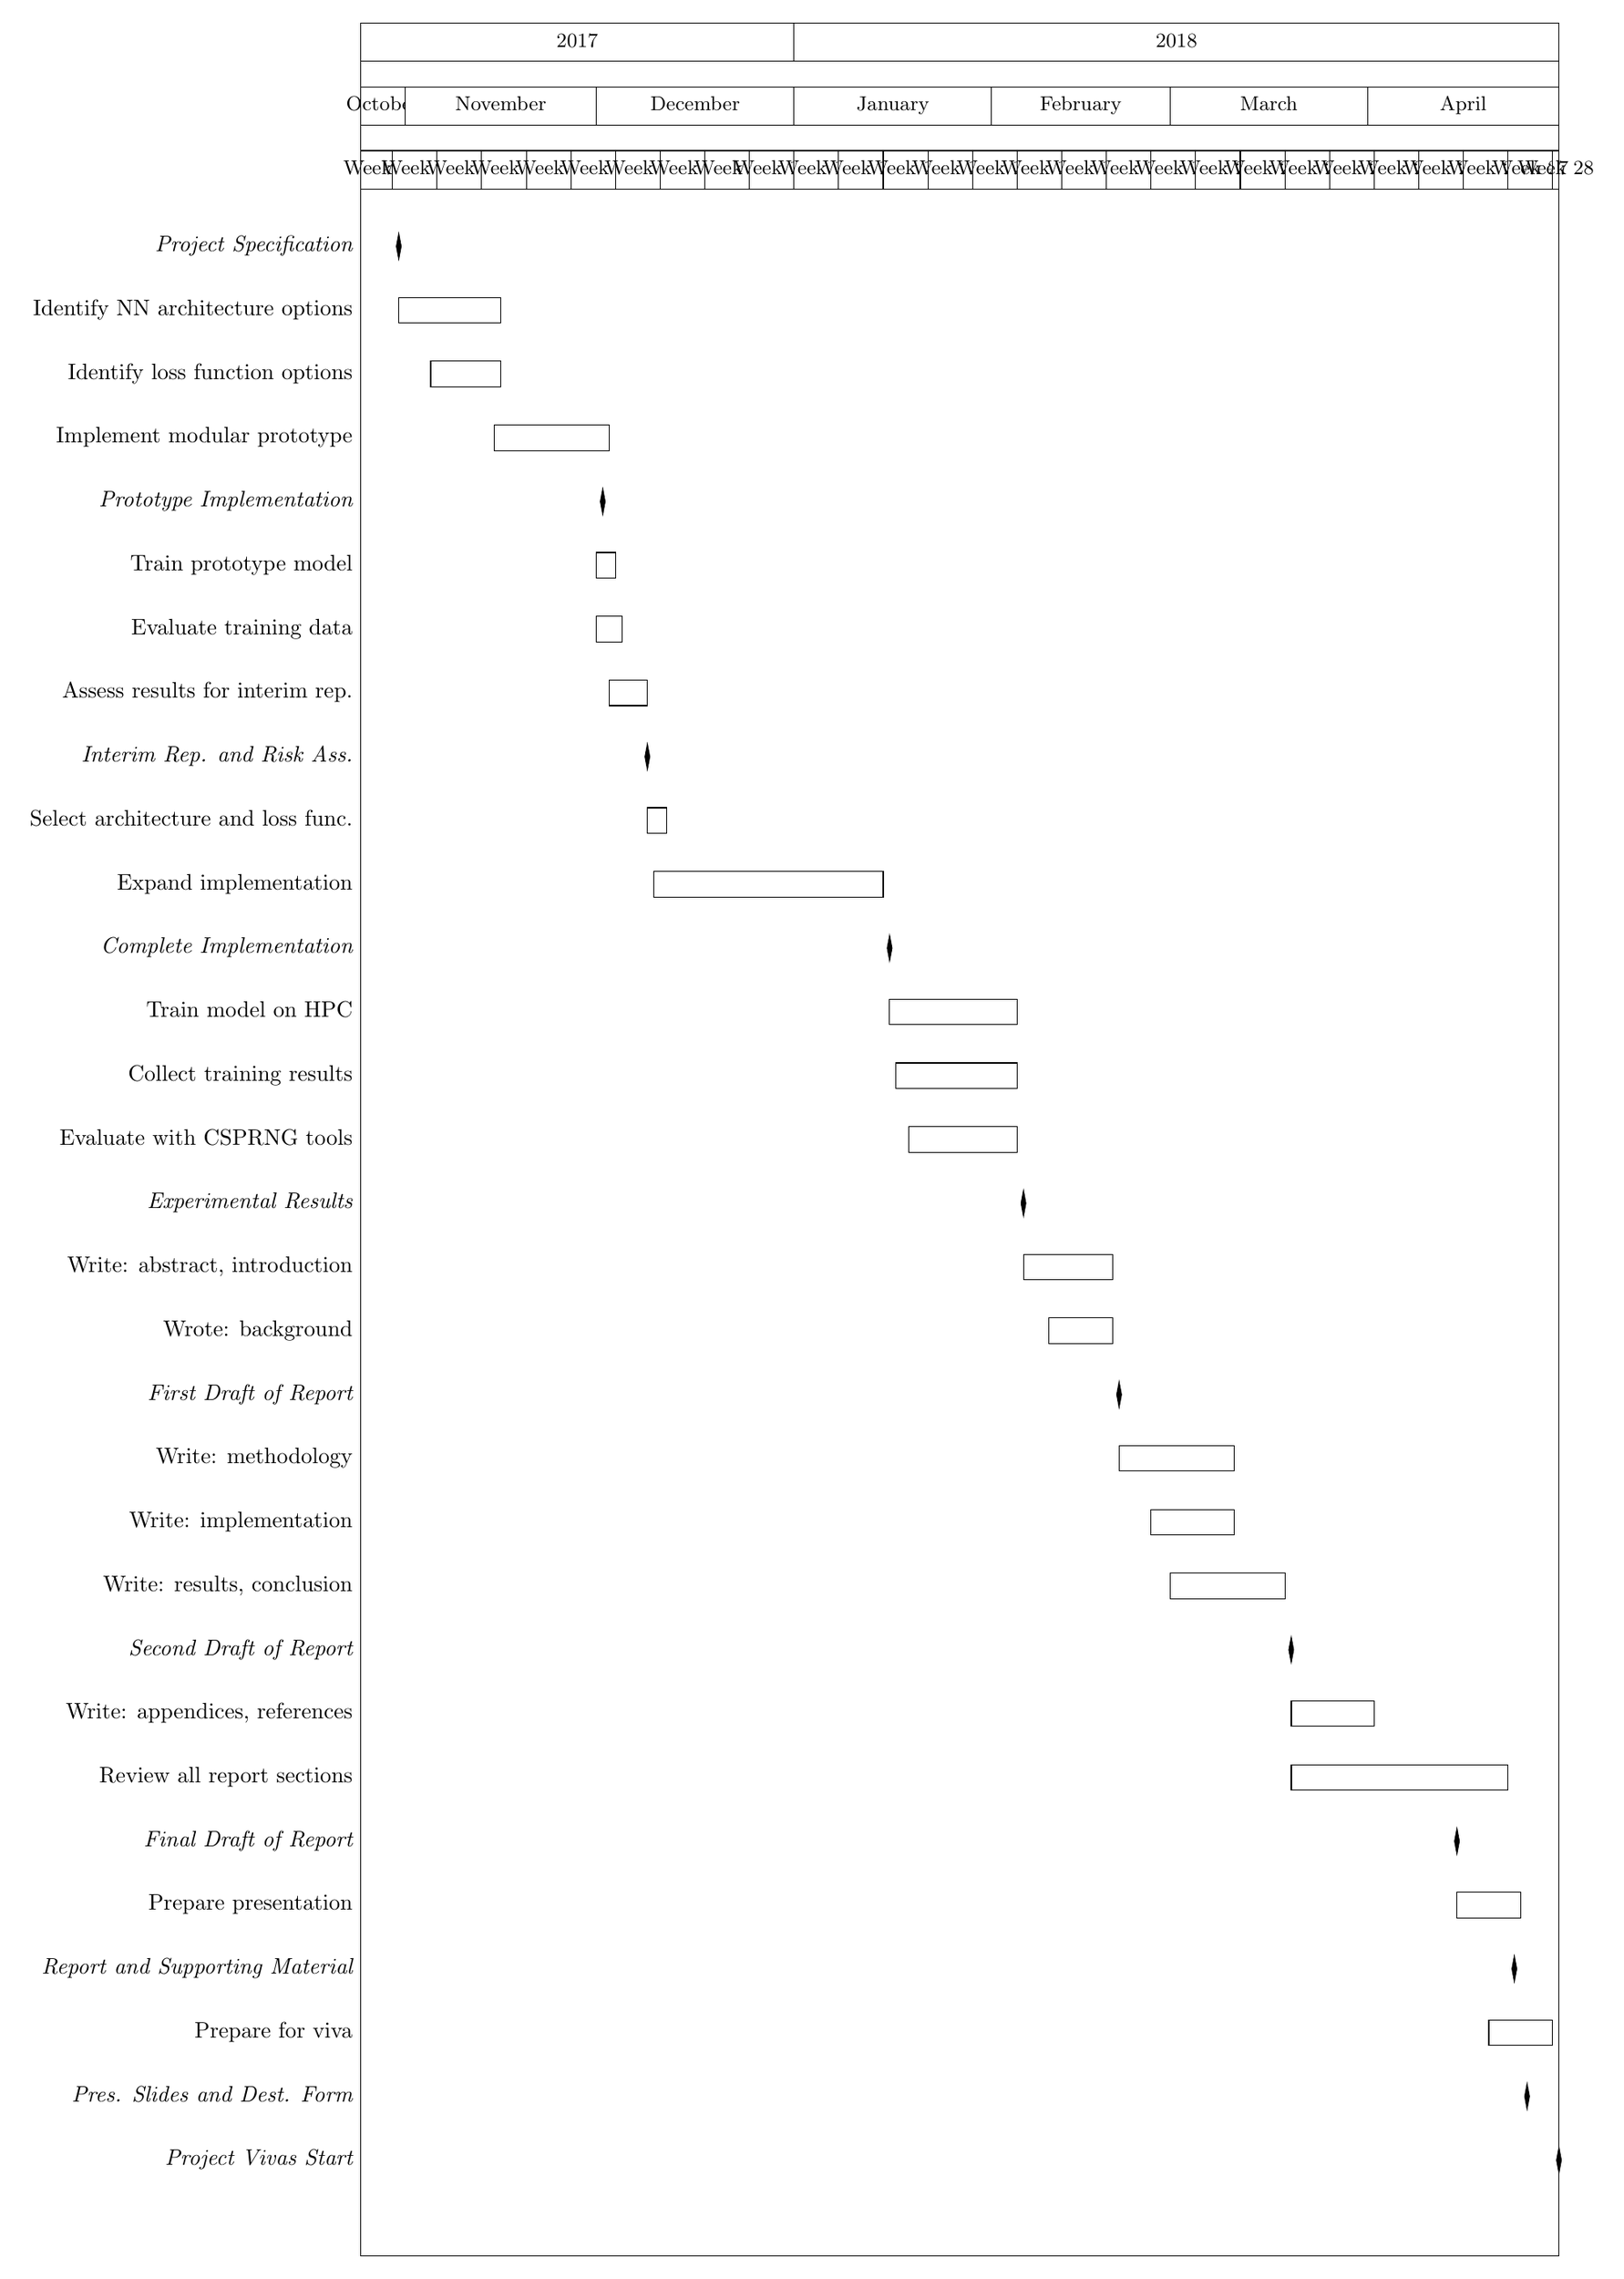
\begin{tikzpicture}
		\begin{ganttchart}[
			x unit=1mm,
			time slot format=isodate-yearmonth,
			time slot format/start date=2017-10-25]{2017-10-25}{2018-04-30}
			\gantttitlecalendar{year, month=name, week} \\
			% \ganttgroup{Group 1}{1}{7} \\
			% \ganttlinkedbar{Task 2}{3}{7} \ganttnewline
			\ganttmilestone{Project Specification}{2017-10-30} \ganttnewline
				\ganttbar{Identify NN architecture options}{2017-10-31}{2017-11-15} \ganttnewline
				\ganttbar{Identify loss function options}{2017-11-05}{2017-11-15} \ganttnewline
				\ganttbar{Implement modular prototype}{2017-11-15}{2017-12-02} \ganttnewline % SPLIT
			\ganttmilestone{Prototype Implementation}{2017-12-01} \ganttnewline
				\ganttbar{Train prototype model}{2017-12-01}{2017-12-03} \ganttnewline
				\ganttbar{Evaluate training data}{2017-12-01}{2017-12-04} \ganttnewline
				\ganttbar{Assess results for interim rep.}{2017-12-03}{2017-12-08} \ganttnewline
			\ganttmilestone{Interim Rep. and Risk Ass.}{2017-12-08} \ganttnewline
				\ganttbar{Select architecture and loss func.}{2017-12-09}{2017-12-11} \ganttnewline
				\ganttbar{Expand implementation}{2017-12-10}{2018-01-14} \ganttnewline % SPLIT
			\ganttmilestone{Complete Implementation}{2018-01-15} \ganttnewline
				\ganttbar{Train model on HPC}{2018-01-16}{2018-02-04} \ganttnewline
				\ganttbar{Collect training results}{2018-01-17}{2018-02-04} \ganttnewline
				\ganttbar{Evaluate with CSPRNG tools}{2018-01-19}{2018-02-04} \ganttnewline
			\ganttmilestone{Experimental Results}{2018-02-05} \ganttnewline
				\ganttbar{Write: abstract, introduction}{2018-02-06}{2018-02-19} \ganttnewline
				\ganttbar{Wrote: background}{2018-02-10}{2018-02-19} \ganttnewline
			\ganttmilestone{First Draft of Report}{2018-02-20} \ganttnewline
				\ganttbar{Write: methodology}{2018-02-21}{2018-03-10} \ganttnewline
				\ganttbar{Write: implementation}{2018-02-26}{2018-03-10} \ganttnewline
				\ganttbar{Write: results, conclusion} {2018-03-01}{2018-03-18} \ganttnewline
			\ganttmilestone{Second Draft of Report}{2018-03-19} \ganttnewline
				\ganttbar{Write: appendices, references}{2018-03-20}{2018-04-01} \ganttnewline
				\ganttbar{Review all report sections}{2018-03-20}{2018-04-22} \ganttnewline
			\ganttmilestone{Final Draft of Report}{2018-04-14} \ganttnewline
				\ganttbar{Prepare presentation}{2018-04-15}{2018-04-24}\ganttnewline
			\ganttmilestone{Report and Supporting Material}{2018-04-23} \ganttnewline
				\ganttbar{Prepare for viva}{2018-04-20}{2018-04-29} \ganttnewline
			\ganttmilestone{Pres. Slides and Dest. Form}{2018-04-25} \ganttnewline
			\ganttmilestone{Project Vivas Start}{2018-04-30} \ganttnewline
			% \ganttbar{Final Task}{8}{12}
			% \ganttlink{elem2}{elem3}
			% \ganttlink{elem3}{elem4}
		\end{ganttchart}
		\end{tikzpicture}
	}
\end{turn}

\bibliographystyle{plain}
\bibliography{references.bib}


\end{document}
